\documentclass[11pt,letterpaper]{article}
\usepackage[hmargin=.77in,vmargin=.65in]{geometry}
\usepackage[T1]{fontenc}
\usepackage{lmodern,graphicx,booktabs,tabularx,amsmath,microtype,float}
\usepackage{tikz}
\usetikzlibrary{arrows.meta,shapes.geometric}
\usepackage[hidelinks]{hyperref}

\newcommand{\shot}[3]{%
  \begin{figure}[H]
    \centering
    \includegraphics[width=#1,height=.76\textheight,keepaspectratio]{figures/#2.png}
    \caption{#3}
    \label{fig:#2}
  \end{figure}%
}
\newcommand{\note}[1]{\par\medskip\noindent #1\par\medskip}
\tikzset{
  box/.style={draw, rounded corners=2pt, align=center, text width=2.18cm, minimum height=10mm, inner sep=3pt},
  decision/.style={draw, diamond, aspect=1.55, align=center, inner sep=2pt},
  route/.style={-{Stealth[length=2mm]}, thick}
}
\hypersetup{pdftitle={GQ Atlas: User Guide and Methods},pdfauthor={The Sonic Waves}}
\title{\textbf{GQ Atlas}\\[.25em]\large User Guide and Methods}
\author{The Sonic Waves}
\date{2026 NASA Space Apps Challenge}
\begin{document}
\maketitle

\begin{abstract}
The Sonic Waves built GQ Atlas for NASA's \emph{Be An Earth System Trend Detective!} challenge. The Atlas turns NASA's gridded temperature record and other Earth science data into an interactive globe, local time series, and statistical tests. One example follows a question from map to evidence: in 2025, how much farther above its own historical average was the Canadian Arctic than Toronto? The guide reproduces that comparison, explains how the Atlas fits and tests trends, and shows how it extends recent patterns through 2100.
\end{abstract}

\begin{center}
\href{https://www.spaceappschallenge.org/2026/challenges/earth-system-trend-detective/}{Be An Earth System Trend Detective!}\\[.4em]
\href{https://gqatlas.vercel.app/}{Live Atlas}
\quad\textbar\quad
\href{https://github.com/advayc/space-apps}{Source code}
\quad\textbar\quad
\hyperlink{demo}{Demo walkthrough}
\end{center}

\shot{.68\linewidth}{globe}{Surface temperature on the Atlas globe. The timeline distinguishes historical values from projections.}
\clearpage
\setcounter{tocdepth}{1}
\tableofcontents

\section{Explore a place}
\begin{figure}[H]
\centering
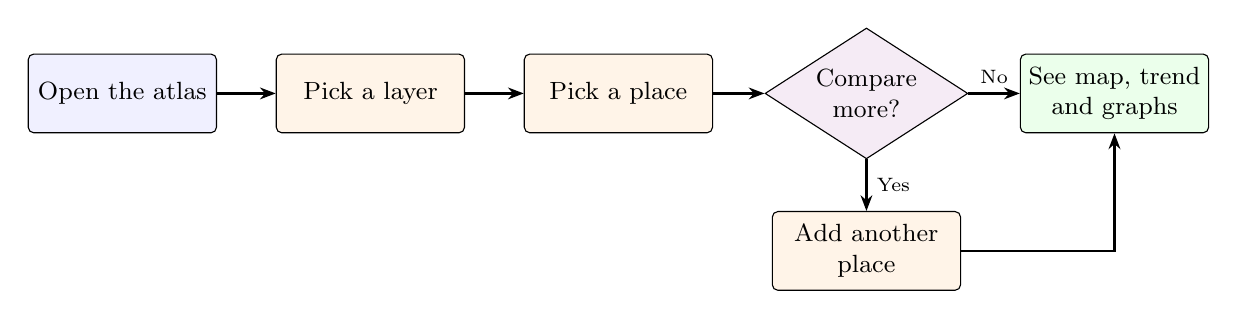
\begin{tikzpicture}[x=1cm,y=1cm,font=\small]
\node[box,fill=blue!6] (start) at (0,0) {Open the atlas};
\node[box,fill=orange!9] (layer) at (3.15,0) {Pick a layer};
\node[box,fill=orange!9] (place) at (6.3,0) {Pick a place};
\node[decision,fill=violet!8] (compare) at (9.45,0) {Compare\\more?};
\node[box,fill=green!8] (results) at (12.6,0) {See map, trend\\and graphs};
\node[box,fill=orange!9] (add) at (9.45,-2.0) {Add another\\place};
\draw[route] (start) -- (layer);
\draw[route] (layer) -- (place);
\draw[route] (place) -- (compare);
\draw[route] (compare) -- node[above,font=\scriptsize]{No} (results);
\draw[route] (compare) -- node[right,font=\scriptsize]{Yes} (add);
\draw[route] (add) -| (results);
\end{tikzpicture}

\caption{Atlas user workflow, redrawn from the team flowchart.}
\label{fig:workflow}
\end{figure}
\begin{enumerate}
\item Open the map or search for a city or coordinates, for example \texttt{43.65, -79.38}. The landing search and the map sidebar both show suggestions. You can also select a spot directly.
\item Choose a climate layer and switch between the flat map and the rotatable globe. Drag to move the view, zoom, or recenter on the selected place. Hover to inspect another cell while the selected place stays marked.
\item Use the year field, slider, arrows, or play button. Annual view shows one value per year. Monthly and seasonal views let you select a shorter period. The 30-year trend view colors the map by rate of change per decade. Violet dates mark projections.
\item Read the small chart in the sidebar or choose \textbf{View larger chart}. Hover to inspect a point, zoom and pan through the record, or select two points to examine their span. The larger chart also has a Monthly view.
\end{enumerate}
\subsection*{Read the colors and numbers}
An anomaly is a difference from a reference average. An anomaly of \(+1.2\,{}^\circ\mathrm{C}\) means a place was 1.2 degrees above its reference average for that period. Use the layer's legend to interpret color and units. Gray marks missing values. The map uses a fixed color scale across dates within each view.
\note{A city label points to a grid cell and describes the surrounding area. Historical averages shows the baseline for the selected period and the mean anomaly across the available record. NASA GISTEMP already supplies anomalies, so its baseline is displayed as zero.}

\clearpage
\hypertarget{demo}{}
\section{Compare places and run a demo}
\noindent\begin{minipage}[t]{.53\linewidth}\vspace{0pt}\raggedright
\textbf{Question.} How far above their own historical averages were the Canadian Arctic and Toronto in 2025?
\begin{enumerate}
\item Select \textbf{Surface temperature anomaly}, \textbf{Annual anomaly}, and \textbf{2025}.
\item Keep Canadian Arctic as the primary place (A). Click \textbf{Compare}, search Toronto, and choose it as B.
\item Read both anomalies and the table's comparison relative to A. Open the larger chart to follow both records, then read the trend significance beside it.
\end{enumerate}
\note{In Figure~\ref{fig:compare}, the Arctic cell was \(+3.45\) and Toronto was \(+1.01\) degrees Celsius relative to their own 1951--1980 baselines. The table shows Toronto at \(-2.44\) degrees relative to A, so the Arctic anomaly was 2.44 degrees larger.}
The places share a layer, period and date. In this example, the 1996--2025 fitted rates were +0.40 and +0.33 degrees Celsius per decade. The Arctic slope had \(p=0.0506\), just above the 5\% cutoff. Add more places with Compare. Remove comparisons individually or clear the set to return to one place.

Atlas compares fitted rates over the same 30 measured years when both records have coverage. The main significance test evaluates the primary cell's slope against zero. Two fitted rates alone cannot establish a statistically significant difference between them.
\end{minipage}\hfill
\begin{minipage}[t]{.44\linewidth}\vspace{0pt}
\shot{\linewidth}{compare}{Canadian Arctic and Toronto in the comparison sidebar.}
\end{minipage}

\shot{\linewidth}{comparison-chart}{Full-size chart of the two annual temperature records.}

\clearpage
\section{From observations to trend estimates}
\begin{figure}[H]
\centering
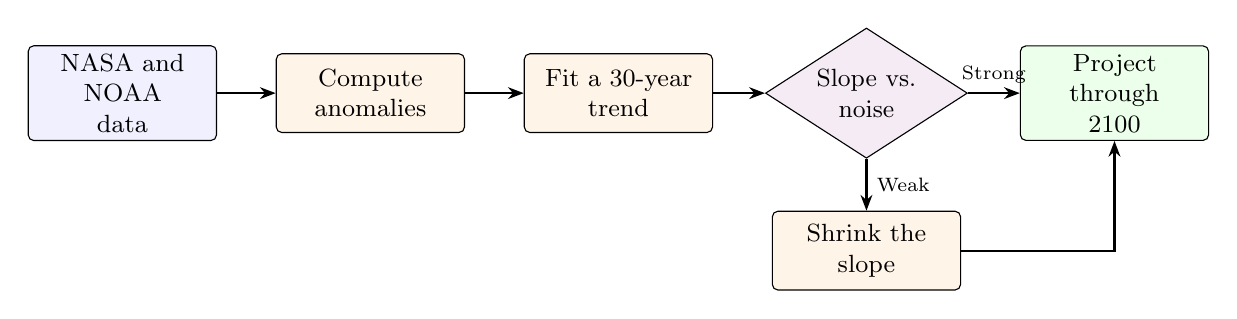
\begin{tikzpicture}[x=1cm,y=1cm,font=\small]
\node[box,fill=blue!6] (data) at (0,0) {NASA and NOAA\\data};
\node[box,fill=orange!9] (anomaly) at (3.15,0) {Compute\\anomalies};
\node[box,fill=orange!9] (fit) at (6.3,0) {Fit a 30-year\\trend};
\node[decision,fill=violet!8] (strength) at (9.45,0) {Slope vs.\\noise};
\node[box,fill=green!8] (projection) at (12.6,0) {Project through\\2100};
\node[box,fill=orange!9] (shrink) at (9.45,-2.0) {Shrink the\\slope};
\draw[route] (data) -- (anomaly);
\draw[route] (anomaly) -- (fit);
\draw[route] (fit) -- (strength);
\draw[route] (strength) -- node[above,font=\scriptsize]{Strong} (projection);
\draw[route] (strength) -- node[right,font=\scriptsize]{Weak} (shrink);
\draw[route] (shrink) -| (projection);
\end{tikzpicture}

\caption{Projection workflow, redrawn from the team flowchart. The decision branch summarizes a continuous adjustment. The displayed 5\% significance test is calculated separately.}
\label{fig:pipeline}
\end{figure}
\subsection*{From a data file to an anomaly}
Figure~\ref{fig:pipeline} summarizes how the records become projections. The Python script reads monthly NetCDF grids. When a product needs a baseline, the script subtracts each cell's reference average for the matching month, season or year. Annual and seasonal means weight each month by its number of days and require complete periods. A December--February season is named for the year containing January and February. Some grids are sampled onto the atlas grid using the nearest source point.

\subsection{Compute the anomaly}
For year \(t\) and a matching period \(p\), let \(z_{t,p}\) denote the source value. Atlas compares it with the historical mean \(\bar z_{\mathrm{ref},p}\) for the same cell and period:
\[
 a_{t,p}=z_{t,p}-\bar z_{\mathrm{ref},p}.
\]
GISTEMP supplies this difference already. When the reference is a 1991--2020 January average, a January anomaly is relative to other Januaries. A chart in this mode follows January across years without mixing it with other months.

\subsection{Fit a line to 30 years}
For one grid cell and period, let \(y_i\) be the anomaly in year \(i\), with \(i=0,\dots,29\). Center the year index by setting \(x_i=i-14.5\). Ordinary least squares chooses the slope \(b\) that minimizes the sum of squared vertical distances to the fitted line:
\[
 \hat y_i=\bar y+b x_i,\qquad
 b=\frac{\sum_i x_i(y_i-\bar y)}{\sum_i x_i^2},\qquad
 \text{trend per decade}=10b.
\]
For example, a slope of \(0.040\,{}^\circ\mathrm{C}\) per year is \(0.40\,{}^\circ\mathrm{C}\) per decade. This calculation describes the fitted rate, even when individual years move up and down. The 30-year trend map and trend panel need consecutive values for this calculation. The interactive chart's interval fit instead describes the span the reader selects.

\subsection{Test the slope}
Atlas uses a Newey--West standard error with three lags~\cite{newey-west} to allow nearby years' errors to be related. If \(s_{\mathrm{NW}}\) is the estimated yearly slope standard error, the approximate 95\% interval per decade is \(10(b\pm1.96s_{\mathrm{NW}})\). The two-sided p-value evaluates how unusual a slope this far from zero would be under a zero-slope hypothesis. Atlas flags \(p<0.05\). A result above the cutoff can reflect a noisy or short record. The app applies the test to the primary grid cell and selected window, without correcting for multiple comparisons across the world map.

\clearpage
\section{How projections through 2100 are made}
\subsection{Extend the trend and damp weak slopes}
Atlas fits the latest 30 measured years for the selected period. In a complete window, let \(S_{xx}=\sum_i x_i^2\), \(e_i=y_i-\hat y_i\), and \(s=\sqrt{\sum_i e_i^2/(30-2)}\). The projection uses the ordinary slope standard error \(s/\sqrt{S_{xx}}\) to calculate \(\tau=b/(s/\sqrt{S_{xx}})\). Atlas applies this weight to the slope:
\[
 w =
 \begin{cases}
 0 & \text{if }|\tau|\le 1,\\
 1-\tau^{-2} & \text{if }|\tau|>1.
 \end{cases}
 \qquad
 \hat y_{\text{future}}(x)=\bar y+w b x.
\]
For instance, a slope twice its standard error keeps 75\% of its fitted value. This is the projection adjustment illustrated in Figure~\ref{fig:pipeline}. The significance panel uses its own Newey--West test.

\subsection{Add year-to-year variation and a prediction range}
The map shows a possible path. For each future year Atlas deterministically chooses a past year in the fitting window and adds that year's residual \(e_i\). Using the same historical index across cells helps retain the spatial pattern of past fluctuations. The central line shows the smoothed estimate. With a complete fit, the shaded prediction half-width at future centered time \(x\) is
\[
 H_k=\min(2,1.25+0.03k)\,(2.0484)\,s
      \sqrt{1+\frac{1}{30}+\frac{x^2}{S_{xx}}},
\]
where \(k=0\) is the first projected year and \(2.0484\) is the 97.5th percentile of Student's \(t\) with 28 degrees of freedom. The multiplier was calibrated using hindcasts. The band is a range for an individual future value, separate from the confidence interval on the fitted historical slope.

\subsection{Work through a projection}
Suppose a complete 1996--2025 fit has a mean anomaly of \(0.60\,{}^\circ\mathrm{C}\), a slope of \(0.04\,{}^\circ\mathrm{C}\) per year, and \(\tau=2\). The fitted midpoint is 2010.5. For 2050, \(x=39.5\) and the adjusted slope is \(0.75\times0.04=0.03\,{}^\circ\mathrm{C}\) per year. The projected central value is \(0.60+0.03\times39.5\approx1.79\,{}^\circ\mathrm{C}\) above the reference average. This example uses hypothetical inputs. An actual cell's estimate and range depend on its 30 values and their variation.

With gaps, Atlas requires at least eight values in the window to fit a slope. It uses the available mean below that threshold, or the last recorded value if there are no values in the window. Incomplete fits do not carry a calibrated range. Neighboring cells can fill remaining gaps on nearly global layers. Land and ocean masks still apply.

\clearpage
\subsection{What the hindcasts tell us}
A hindcast gives the algorithm only data available before a historical cutoff, then checks the estimate against later values already in the record. The project's \href{https://gqatlas.vercel.app/projections/}{Projections page} reports that about 93--98\% of later observations fell inside the adjusted bands across layers. It also reports that the temperature trend improved only slightly on a flat baseline and that other variables had no meaningful improvement. These checks describe the tested historical windows. They do not establish coverage for a different climate regime or the year 2100.

\shot{\linewidth}{projection}{The Atlas Projections page shows the historical global temperature series, the recent fit, and the widening range.}

\subsection{Read a projected value}
Start with the measured record to see whether change persists across years. Then use the projected line to ask what continued change might look like. In Figure~\ref{fig:projection}, the Atlas's global surface-temperature calculation puts the 2100 central estimate at \(+2.99\,{}^\circ\mathrm{C}\), with a range of \(+2.10\) to \(+3.88\,{}^\circ\mathrm{C}\), relative to 1951--1980. Look at the band before quoting a late-century value: the width grows as the method extrapolates farther. The global average combines many cells and is usually smoother than a single location. The Projections page gives an illustrative spread around 2100 of roughly \(\pm0.9\,{}^\circ\mathrm{C}\) globally and \(\pm3.6\,{}^\circ\mathrm{C}\) for a typical cell. Local ranges vary. The Atlas fits past values and does not include future emissions pathways, physical feedbacks or policy changes. Use assessed climate-model scenarios for decisions that depend on future conditions.

\clearpage
\section{Compare variables and explore hydrology}
\textbf{Scatter plot.} Use the preset arrows or choose X and Y separately. Every dot represents a year with valid measured values for both variables at the selected place. Hover to read the values and year. Pearson's \(r\) describes the strength and direction of a straight-line relationship, from \(-1\) to \(+1\).

\textbf{Remove long-term trends.} Use the checkbox to see how the variables move together after removing each series' fitted trend. Correlation alone cannot establish cause. Land-only and ocean-only layers may have no overlapping values.
\shot{.74\linewidth}{scatter}{Scatter plot with the temperature and precipitation preset.}

\subsection*{Try a two-variable investigation}
Ask whether warmer years at your selected cell also tend to be wetter. Choose the temperature and precipitation preset, check how many years overlap and note their correlation. Turn on detrending and compare the result with the first one. Export the paired values if you want to check unusual years or reproduce the comparison elsewhere. If both variables have long-term trends, compare the two results before interpreting the relationship.
\clearpage
\subsection{NASA hydrology viewer}
Select a place on land, choose a GLDAS variable and date range, and click \textbf{Download NASA CSV}. NASA may ask for an Earthdata Login. Open the file in Atlas to plot the series locally in the browser. The chart keeps the file's units, variable and coordinates.
\shot{\linewidth}{hydrology}{The hydrology controls. Requests and imported charts are separate from the map layers.}
The five options cover topsoil moisture, root-zone soil moisture, evapotranspiration, precipitation rate and snow water equivalent. GLDAS estimates land conditions with a model. Masked water cells have no values.

\section{Datasets and coverage}
These dates describe complete annual periods in the atlas snapshot. Monthly availability varies. Every map layer links to its product page and original file in \textbf{Where this data comes from}.

\noindent{\small\renewcommand{\arraystretch}{1.25}%
\begin{tabularx}{\linewidth}{@{}>{\raggedright\arraybackslash}p{.27\linewidth}>{\raggedright\arraybackslash}Xl@{}}
\toprule
\textbf{Product} & \textbf{What Atlas uses} & \textbf{Annual dates}\\
\midrule
\href{https://data.giss.nasa.gov/gistemp/data_v4.html}{NASA GISS GISTEMP v4} & Land--Ocean Temperature Index. Surface temperature anomaly, \texttt{tempanomaly}, in degrees Celsius. & 1880--2025\\
\href{https://psl.noaa.gov/data/gridded/data.gpcp.html}{NOAA PSL GPCP v2.3} & Satellite and gauge precipitation, in mm/day. & 1979--2025\\
\href{https://psl.noaa.gov/data/gridded/data.noaa.ersst.v6.html}{NOAA PSL ERSST v6} & Reconstructed sea surface temperature, in degrees Celsius. & 1850--2025\\
\href{https://psl.noaa.gov/data/gridded/data.ncep.reanalysis.html}{NCEP/NCAR Reanalysis 1 via NOAA PSL} & Air and skin temperature, water vapor, sea level pressure, wind speed and two components, cloud cover, topsoil moisture and temperature, incoming sunlight, latent and sensible heat flux, and outgoing longwave radiation. & 1948--2025\\
\href{https://psl.noaa.gov/data/gridded/data.noaa.oisst.v2.html}{NOAA OISST v2} & Sea ice concentration anomaly, in percentage points. & 1982--2022\\
\bottomrule
\end{tabularx}%
}\par
\subsection*{NASA dataset details}
\textbf{GISTEMP v4.}~\cite{gistemp} Atlas uses the monthly 2-degree NetCDF grid with 1,200 km smoothing and a 1951--1980 reference. NASA combines land air observations and ocean surface temperature estimates in its Land--Ocean index. This grid drives the temperature map, place records and trends. The landing chart uses an area-weighted global mean of the annual grid. \href{https://data.giss.nasa.gov/pub/gistemp/gistemp1200_GHCNv4_ERSSTv5.nc.gz}{Exact NetCDF download}.

\textbf{GLDAS-2.1 Noah monthly.}~\cite{gldas} The optional explorer requests \texttt{GLDAS\_NOAH025\_M} v2.1 model estimates at selected coordinates on a 0.25-degree land grid, with records beginning in 2000. The \href{https://disc.gsfc.nasa.gov/information/tools?title=Hydrology%20Time%20Series}{GES DISC Hydrology Time Series tool} and Giovanni API support point-series access. The model data are plotted after CSV import.

\note{The NOAA-distributed anomaly layers use 1991--2020 cell baselines. A difference of one percentage point means, for example, a change from 20\% to 21\%. The \href{https://gqatlas.vercel.app/data-and-methods/}{Data and methods page} lists references and describes the treatment of missing data.}


\clearpage
\section{What the trends mean for people and ecosystems}
The Atlas trend panel translates a local rate into plain language and links to the broader \href{https://gqatlas.vercel.app/impacts/}{Impacts page}. The examples below suggest questions to investigate with the map and the underlying data.

\begin{description}
\item[Heat and water.] Use the temperature trend to identify regions where warmer conditions warrant a closer look. Then compare precipitation and soil moisture. Annual averages can hide seasonal water shortages or extreme heat. Examine the relevant month or season and consult daily records for extremes.
\item[Ice and Arctic habitats.] Sea ice concentration measures the fraction of an ocean cell covered by ice. It can help frame questions about polar bear habitat, coastal access and seasonal change. Compare the same season across years and avoid treating a local concentration value as total Arctic ice extent.
\item[Wildfires and coastal ecosystems.] Hot or dry periods can make conditions more favorable for wildfire. Satellite smoke imagery documents a specific event and does not attribute it to a particular trend. Warmer surface waters can contribute to coral heat stress, while actual bleaching risk depends on exposure duration and local conditions.
\item[Animals on the move.] Temperature and habitat changes can shift the timing of migration and the range of suitable habitat. The site's animal examples illustrate questions about Arctic foxes, polar bears and seabirds. To test a range shift, compare the climate series with independent observations of where and when the species occurs.
\end{description}

\subsection{How this addresses NASA's challenge}
The project turns NASA GISTEMP into a way to ask a testable question about a local record. A reader chooses a layer, compares places on a shared timeline, checks the slope and uncertainty, and can download the data to reproduce the result. The NASA GLDAS explorer lets readers ask whether modeled soil or water conditions tell a related story. NOAA layers broaden the questions readers can explore. The map shows where change occurs, the slope gives its direction and rate, and the confidence interval and p-value show how well that slope is supported. This brings data discovery, visualization and significance testing together for the \href{https://www.spaceappschallenge.org/2026/challenges/earth-system-trend-detective/}{NASA Space Apps challenge}.

\noindent\begin{minipage}[t]{.52\linewidth}\vspace{0pt}\raggedright
\textbf{Example investigation.} Compare the Canadian Arctic and Toronto with GISTEMP. Record the years and baseline, then distinguish the difference in 2025 anomalies from the fitted rates. Check sea ice in the same season and region as a follow-up. A teacher can use this exercise to show how a mapped pattern becomes a reproducible question about Earth system change. Regional research can help explain the pattern.
\end{minipage}\hfill
\begin{minipage}[t]{.44\linewidth}\vspace{0pt}
\shot{\linewidth}{arctic-impacts}{Arctic satellite mosaic from the Atlas Impacts page. \href{https://commons.wikimedia.org/wiki/File:Mosaic_of_the_Arctic.jpg}{Image credit and source (NASA Earth Observatory)}.}
\end{minipage}

\clearpage
\section{Reproduce, share and credit the work}
\subsection*{Export an analysis}
Download the primary place's values and fit as CSV or download the trend statistics as JSON. Save the map and full chart as PNGs. The scatter panel exports paired annual data as its own CSV. Include the layer, place, date and reference period when sharing a figure so others can interpret it.

\subsection*{Tools and architecture}
\begin{description}
\item[Browser] HTML, CSS and JavaScript provide the interface. Canvas draws the maps and analytical charts. SVG draws the landing chart. D3 Geo, D3 Array and TopoJSON Client support the geographic views.
\item[Preparation] Python, NumPy and netCDF4 transform source files into compact grids. The \href{https://github.com/advayc/space-apps/blob/main/dist/assets/catalog.json}{data catalog} records source variables, URLs, units, years and grid dimensions. The \href{https://github.com/advayc/space-apps/blob/main/scripts/prepare_data.py}{preparation script} defines the transformations.
\item[Hosting] GitHub holds the code and versioned binary grids. Vercel serves the static site. The build excludes the large grids, which the browser fetches from a pinned public GitHub revision. For local use, run \texttt{python3 -m http.server 8080 --directory dist} from the Atlas repository.
\item[Hardware] Development used a laptop. The site runs in web browsers on computers and phones.
\end{description}
\subsection*{Credits and AI use}
The Sonic Waves built GQ Atlas for NASA Space Apps. The interface screenshots come from the Atlas website running locally. The two vector diagrams were redrawn from team-supplied flowcharts. Copies of the supplied diagrams are included with the source. The basemap uses Natural Earth through World Atlas. Third-party library notices are kept with the site assets. The site uses Bricolage Grotesque, IBM Plex Sans and IBM Plex Mono from Google Fonts. Some legacy place and boundary files lack recorded source versions.

The project's submission notes credit Cursor and Anthropic Claude for earlier development. OpenAI Codex assisted with implementation, browser checks and this guide. Atlas computes its numeric results using dataset values and fixed statistical formulas.
\subsection*{Further investigations}
Try comparing two familiar locations, checking whether an unusual year is part of a longer trend, or testing how local water and temperature records move together. Future work includes emissions scenarios, extreme-day counts, finer spatial detail and links that reopen a view.

\href{https://gqatlas.vercel.app/}{Live project}
\quad\textbullet\quad
\href{https://gqatlas.vercel.app/impacts/}{Impacts}
\quad\textbullet\quad
\href{https://gqatlas.vercel.app/data-and-methods/}{Data and references}
\quad\textbullet\quad
\href{https://github.com/advayc/space-apps}{Source repository}

\begingroup\small
\begin{thebibliography}{9}
\bibitem{gistemp} NASA Goddard Institute for Space Studies.
\href{https://data.giss.nasa.gov/gistemp/}{GISS Surface Temperature Analysis (GISTEMP v4)}. Accessed November 15, 2026.
N. Lenssen et al. \href{https://doi.org/10.1029/2023JD040179}{A GISTEMPv4 observational uncertainty ensemble}. \textit{Journal of Geophysical Research: Atmospheres}, 129(17), 2024.
\bibitem{gldas} NASA Goddard Earth Sciences Data and Information Services Center.
\href{https://ldas.gsfc.nasa.gov/gldas/dataset}{Global Land Data Assimilation System datasets}.
\bibitem{newey-west} W. K. Newey and K. D. West.
A simple, positive semi-definite, heteroskedasticity and autocorrelation consistent covariance matrix.
\textit{Econometrica}, 55(3), 703--708, 1987.
\href{https://doi.org/10.2307/1913610}{doi:10.2307/1913610}.
\bibitem{atlas-methods} The Sonic Waves.
\href{https://gqatlas.vercel.app/data-and-methods/}{GQ Atlas Data and Methods}.
\end{thebibliography}
\endgroup
\end{document}
